\documentclass[12pt, a4paper, titlepage]{report}

    %Germanish stuff
    \usepackage[utf8]{inputenc}
    \usepackage[T1]{fontenc}
    \usepackage{ngerman}

    % Seitenränder
    \usepackage{geometry}
    \geometry{a4paper, top=25mm, left=25mm, right=45mm, bottom=20mm, headsep=10mm, footskip=10mm}

    % 1 1/2 Zeilig
    \usepackage[onehalfspacing]{setspace}

    % Change Font to Arial
    \renewcommand{\familydefault}{\sfdefault}
    \usepackage{uarial}

    % Kopfzeilen, Nummerierung aus für Seiten 1+2
    \usepackage{fancyhdr}
    \lhead{Julian Tölle}
    \chead{\thepage}
    \rhead{Facharbeit}
    \cfoot{}
    \renewcommand{\headrulewidth}{0.4pt}

    \pagestyle{fancy}
    % Fix for Chapter pages:
    \usepackage{etoolbox}
    \patchcmd{\chapter}{\thispagestyle{plain}}{\thispagestyle{fancy}}{}{}

    %\usepackage{bibgerm}
    \usepackage[backend=biber,
    			style=verbose,
    			sortlocale=de_DE,
    			language=german,
    			citestyle=authoryear,
    			dateabbrev=false]{biblatex}
    %\usepackage[babel, german=guillemets]{csquotes}
	\addbibresource{bibindex.bib}
	
	\usepackage[htt]{hyphenat}
	
	\usepackage{url}

%%% --- The following two lines are what needs to be added --- %%%
\setcounter{biburllcpenalty}{7000}
\setcounter{biburlucpenalty}{8000}
	

\usepackage{graphicx}
\begin{document}

    \begin{titlepage}
        \title{Verspricht die Sell-In-May-Anlagestrategie Erfolg?\\
                –\\
                Entwicklung eines Algorithmus zur Lösung dieses Optimierungsproblems
                und der Datenanalyse anhand des Beispiels der Dax-Börsendaten}
        \author{Julian Tölle\\
                Ev. Gymnasium Werther\\
                Informatik-Grundkurs\\
                Herr Möllenbrock}
        \date{Schuljahr 2014/15}

        \maketitle
    \end{titlepage}

    \tableofcontents
    % No header for ToC
    \thispagestyle{empty}

    % Correct page numbering
    \setcounter{page}{2}

    \chapter{Einführung ins Thema}
        
        \section{Der Deutsche Aktienindex}
            Der DAX, kurz für Deutscher Aktienindex, wurde im Jahr 1988 erstmalig
            veröffentlicht, und beinhaltet die 30 größten und umsatzstärksten Aktien
            Deutschlands. Er basierte zu Beginn auf den Kursen der Frankfurter
            Wertpapierbörse, seit dem 21. Juni 1999 bildet die elektronische Börse
            XETRA (Exchange Electronic Trading) die Datengrundlage.
            
            Damit ein Unternehmen in den DAX aufgenommen wird, muss es mehrere Kriterien
            erfüllen. Zuerst muss das Unternehmen im Prime Standard der Frankfurter Börse
            gelistet sein, dies ist ein stärker regulierter Bereich der Börse der hohe
            Transparenzvoraussetzungen erfüllen muss
            \footcite[Vgl.][]{deutscheboersePrimeStandard}.
            Das nächste Kriterium ist, dass das Unternehmen durchgehend auf XETRA
            gehandelt wird. XETRA ist das elektronische Handelssystem der Deutsche
            Börse AG. Es übernimmt die gesamte Verwaltung des Handels, sodass die
            Aufträge schneller als manuell abgearbeitet werden und in hoher Frequenz
            neue Kurse bereitgestellt werden können\footcite[Vgl.][]{boerseFrankfurtXetra}.
            Die letzte Bedingung ist ein Streubesitz von über 10\%. Als Streubesitz
            wird der Teil der Aktien einer AG genannt, die nicht als große Pakete
            wenigen Großaktionären gehören, sondern frei an der Börse gehandelt werden
            \footcite[Vgl.][]{gablerFreefloat}.  
            
            Der DAX ist -- anders als die meisten anderen großen Aktienindizes
            (Dow Jones Industrial Average, FTSE, Nikkei 225) -- ein Performanceindex,
            was bedeutet, dass bei der Berechnung so getan wird als ob alle Dividenden
            und sonstige Einnahmen aus dem Besitz (z.B. Bezugsrechterlöse) von Aktien
            wieder in diese Aktien reinvestiert würden. Üblicherweise sinkt der Wert
            einer Aktie, die eine Dividende an ihre Aktionäre ausschüttet, um eben
            diesen Betrag, ein Kursindex würde also nach der Dividendenausschüttung an
            Punkten verlieren, der DAX allerdings nicht, da der Dividendenabschlag
            durch die positive Bewertung der Auszahlung ausgeglichen wird.
            
            % Was ist der Dax
            % Abgrenzung zu anderen Aktienindizes
            % Gründung
            % Handelsort
            % Auswahl der Wertpapiere

        \section{Sell-in-May als Anlagestrategie}
            \begin{quote}
                Sell in May and go away, but remember to come back in September.
            \end{quote}
            So lautet eine alte Börsenweisheit, die sich darauf bezieht dass es
            in den Wintermonaten eine erheblich höhere Rendite für Anlagen gibt
            als in den Sommermonaten. Nach ihr ist es am effektivsten im Mai alle
            aktuell gehaltenen Aktien zu verkaufen und im September wieder anzuschaffen,
            um so den durchschnittlichen Wertverlust der Aktien im Sommer abzuwarten
            und dann, wenn die Kurse am niedrigsten sind, günstig einzukaufen.

            Der Effekt wurde nur geringfügig wissenschaftlich untersucht, eine
            Studie ist allerdings zu dem Urteil gekommen dass er in 36 von 37
            untersuchten Ländern nachweisbar war\footcite[Vgl.][]{bouman2002halloween}.
            Um dies zu belegen, wurde die Rentabilität einer ''Buy and Hold Strategy``
            mit der Sell-in-May Anlagestrategie für alle untersuchten Märkte über
            mehrere Jahre verglichen. Dies ergab, dass das Sell-in-May Verfahren 
            durchschnittlich 1,5\%, im Hinblick auf die jährliche Rendite, besser
            war als die Aktien dass ganze Jahr zu halten\footcite[Vgl.][S. 14 Tabelle A1]{bouman2002halloween}.
            % Sell in May and go away but remember to come back in september
            % Bisherige Studien zu dem Thema

        \section{Problemstellung}
            Die Zeitspanne eines Monats als Zeitraum für den Verkauf und Einkauf
            der Aktien ist sehr grob. Er gibt keinen Aufschluss über die besten
            Tageskombinationen, sondern nur eine grobe Richtung bei der es zu
            unsicher ist ihr blind zu folgen. Und wo genau der maximale Profit
            steckt, weiß auch keiner so richtig. Magere 1,5\% verspricht die
            vorher erwähnte Studie. Es wird Zeit, dass man diese Rendite maximiert.
            
            Da Marktvorhersagen allerdings nur schwer möglich sind, richten wir
            in dieser Facharbeit unser Augenmerk auf die vergangenen Jahre und 
            schreiben einen Algorithmus der die, historisch gesehen, optimalsten Tage
            für den Kauf und Verkauf der Aktien berechnet. In der Auswertung dieser
            Daten wird dann eine mögliche Tendenz gesucht, die die zukünftigen
            Investitionen vereinfachen soll.
            Als zu betrachtenden Kurs verwende ich den DAX, da er der bekannteste und
            meistgenutzte Indikator für die deutsche Aktienlandschaft ist.
            % Anwendung von Sell-in-May auf den Dax
            % Optimale Tage für die letzten Jahre
            % -> Optimierungsproblem

    \chapter{Anforderungsanalyse}
        \section{Frontend}
        	\subsection{\texttt{com.toelle.maytoseptember.view}}
        		Das Frontend soll eine grafische Oberfläche (GUI) bieten, über die
        		Aktien geladen, sowie Parameter zur Optimierung eingestellt werden 
        		können. Verfügbare Informationen zur geladenen Aktie, wie beispielsweise
        		die Anzahl, der Name oder die Zeitspanne der Einträge sollen angezeigt
        		werden. Gleiches gilt für die Optimierung, wo die Zeitspannen zum 
                Verkauf und Ankauf, die errechneten optimalen Tage und der Performance
                Index angezeigt werden.
        		
        		Im GUI sollte auch ein Graph vorhanden sein, der den zeitlichen Verlauf
        		der Aktie sowie den theoretischen Verlauf unter Beachtung der
        		optimalen Kauf- und Verkauftage darstellt.

        \section{Backend}
        	\subsection{\texttt{com.toelle.maytoseptember.model}}
        		Das \texttt{model} Package beinhaltet die Klassen zur Modelierung der
        		Daten. Im folgenden wird auf die Funktion der einzelnen Klassen genauer
        		eingegangen, da diese Darstellungsform die Übersicht vereinfacht.
        		
        		\subsubsection{\texttt{com.toelle.maytoseptember.model.Date}}
        		Diese Klasse repräsentiert einen einzelnen Tag, durch die drei
        		Felder \texttt{int day}, \texttt{int month} und \texttt{int year}.
        		
        		Sie hat eine Konstruktormethode die aus einem String mit dem Format
        		\texttt{YYYY-MM-DD} ein entsprechendes \texttt{Date} Objekt erzeugt.
        		
        		Sie implementiert das Interface \texttt{Comparable} damit man mehrere
        		\texttt{Date} Objekte miteinander vergleichen kann.
        		
        		Sie implementiert eine Methode \texttt{next()} mit der man zuverlässig
        		aus dem aktuellen Tag den nächsten Tag generieren kann.
        		
        		\subsubsection{\texttt{com.toelle.maytoseptember.model.DateRange}}
        		Diese Klasse repräsentiert eine Zeitspanne, die sich durch ein Anfangs-
        		sowie ein Enddatum auszeichnet.
        		
        		Sie implementiert eine Methode \texttt{getContainedDates()} die
        		ein \texttt{List<Da\allowbreak te>} Objekt, bestehend aus allen Tagen die zwischen
        		dem Anfangs- und dem Enddatum sind zurückgibt.
        		
        		Sie implementiert eine Methode \texttt{isInRange()}, welche unter Angabe
        		des zu überprüfenden \texttt{Date} Objekts ermittelt ob es sich innerhalb
        		der Zeitspanne, es wird \texttt{true} zurückgegeben, oder außerhalb, es
        		wird \texttt{false} zurückgegeben, befindet.
        		
        		Sie implementiert eine Methode \texttt{isInYearlyRange()}, welche unter
        		Angabe des zu überprüfenden \texttt{Date} Objekts ermittelt, ob es sich
        		innerhalb oder außerhalb der Zeitspanne befindet, dabei ist das Jahr egal,
        		und es kommt nur auf den Tag und den Monat an.
        		
        		\subsubsection{\texttt{com.toelle.maytoseptember.model.StockData}}
        		Diese Klasse repräsentiert die Daten für einen Tag der Aktie. Sie besteht
        		aus den zwei Feldern \texttt{BigDecimal value} und \texttt{Date date}.
        		
        		\subsubsection{\texttt{com.toelle.maytoseptember.model.StockHistory}}
        		Diese Klasse beinhaltet eine sortierte \texttt{Map} für die
        		zeitliche Abfolge von \texttt{StockData} Objekten. Der Schlüssel
        		ist das \texttt{Date} und der Wert jedes Eintrags ist das zugehörige
        		\texttt{StockData} Objekt.
        		
        		Sie implementiert eine Methode \texttt{getStockData()} die unter
        		Angabe des \texttt{Date} Objekts das zugehörige \texttt{StockData}
        		Objekt zurückliefert.
        		
        		\subsubsection{\texttt{com.toelle.maytoseptember.model.Stock}}
        		Diese Klasse besteht aus den Feldern \texttt{String name} und
        		\texttt{StockHistory history} und repräsentiert eine Aktie.
        		
        		\subsubsection{\texttt{com.toelle.maytoseptember.model.OptimizedStock}}
        		Diese Klasse repräsentiert den Zusammenschluss aus einem \texttt{Stock}
        		Objekt und seinen Optimierungsinformationen. Es enthält die Felder
        		\texttt{Stock optimizedStock}, \texttt{DateRange sellingTime},
        		\texttt{DateRange buyingTime}, \texttt{Date[] optimalDates}, 
        		\texttt{float performanceIndex} und \texttt{boolean optimized}.
        		
        		Das Attribut \texttt{optimized} beschreibt, ob das Objekt für
        		seine aktuelle Konfiguration in den Feldern \texttt{optimalDates}
        		und \texttt{performanceIndex} optimierte Daten beinhaltet. Dies
        		kann über die Methode \texttt{isOptimized()} abgefragt werden.
        		
        		Sie implementiert eine Methode \texttt{setOptimizedData()} mit den
        		Parametern \texttt{Date[] optimalDates} und \texttt{float performanceIndex}
        		die beide Felder ändert. Es ergibt Sinn eine Änderung an dem einen
        		nur dann zuzulassen, wenn das andere auch geändert wird, da sonst
        		inkonsistente Zustände auftreten können. Auch wird durch diese Methode
        		das \texttt{optimized} Flag auf \texttt{true} gesetzt.        		
        	
        	\subsection{\texttt{com.toelle.maytoseptember.controller}}
        		Dieses Package beinhaltet Klassen die auf den Daten aus dem
        		\texttt{model} Package arbeiten, sowie aus
        		einer weiteren Klasse zum anfertigen von Logs.
        		
        		\subsubsection{\texttt{com.toelle.maytoseptember.controller.Logger}}
        		Diese Klasse besteht aus einer einzigen statischen Methode
        		\texttt{log()}, die als Parameter \texttt{String msg} und
        		\texttt{LoggingLevel level} erwartet. Abhängig von \texttt{level} wird
        		die \texttt{msg} in der Konsole ausgegeben und in die Log Datei
        		geschrieben.
        		
        		\subsubsection{\texttt{com.toelle.maytoseptember.controller.DatabaseConnection}}
        		Diese Klasse ist dafür zuständig, die Daten, wie den Namen der Aktie und ihren
        		Verlauf, aus der MySQL Datenbank zu holen und aufzubereiten, damit sie als
        		Objekte von Klassen aus dem \texttt{model} Package bereitstehen.
        		
        		Der Konstruktor lädt den JDBC Treiber des Systems und baut eine Verbindung
        		zur Datenbank auf.
        		
        		Die Methode \texttt{getStockFromDatabase()} erstellt ein vollständiges
        		\texttt{Stock} Objekt mit dazugehöriger \texttt{StockHistory}, basierend auf
        		den Daten aus der Datenbank, und gibt dieses zurück.
        		
        		\subsubsection{\texttt{com.toelle.maytoseptember.controller.StockOptimizer}}
        		Diese Klasse ist für die Berechnung der optimalen Tageskombination
        		zum Kauf und Verkauf der Aktie zuständig.
        		
        		Sie implementiert die statische Methode \texttt{optimize()} die als 
        		Parameter ein \texttt{OptimizedStock} Objekt erwartet, bei dem die
        		\texttt{sellingRange} und \texttt{buyingRange} bereits gesetzt sind.
        		Sie gibt das selbe Objekt wieder zurück, allerdings nun mit gesetzten
        		Optimierungsergebnissen.
        		
        		Auf die Funktionsweise dieser Klasse wird in Kapitel 3 genauer eingegangen.

    \chapter{Entwicklung des Algorithmus}

        \section{Algorithmische Grundidee}
            Der Algorithmus berechnet die Lösung durch eine Bruteforcing Methode.
            Bruteforcing besteht auf der Idee dass, obwohl es keinen
            effizienten, und möglicherweise komplizierteren, Algorithmus gibt, man
            einfach alle Optionen ‘‘ausprobiert'' und die beste auswählt. Dies kann
            allerdings auch dazu führen dass die Laufzeit des Algorithmus bei großen
            Datenmengen weit über der eines effizienteren Algorithmus liegen kann.
            Da sich die Fragestellung allerdings nur im Bereich von wenigen Millionen
            Rechnungen\footnote{$30~(Tage~im~Mai) * 31~(Tage~im~September) * 4370~
            (Tageskurse) = 4.064.100$} befindet, ist Bruteforcing eine brauchbare
            Alternative zu der Entwicklung eines alternativen Algorithmus.
   			Für eine extensive Nutzung des entwickelten Programms allerdings sollte
   			er noch weiter optimiert werden.

            Zu Beginn wird eine Liste, bestehend aus jeder durchzurechnenden Option,
            erstellt, jedes Element dieser Liste besteht aus zwei Tagen. Der erste Tag 
            kommt aus der Zeitspanne zum Verkauf, hier also aus dem Mai, der zweite
            Tag kommt aus der Zeitspanne zum Einkauf, hier also aus dem September.
            Für jede mögliche Kombination der Elemente dieser beiden Listen gibt es
            einen Eintrag in der neu erstellten Liste.

            Nun wird für jede Kombination ihrer Rentabilität in Form eines
            Performance Indexes berechnet. Dies geschieht indem mit Hilfe eines
            simulierten Depots der Weg des Geldes nachgestellt wird.
            Am Anfang gibt es eine bestimmte Geldmenge, und nun werden alle
            geladenen Tageskurse des DAX chronologisch durchlaufen.
            Falls sich das Datum des Tageskurses zwischen Verkauf
            und Kauf befindet, werden alle noch im Depot vorhandenen Aktien
            verkauft, und falls es sich außerhalb dieser Zeitspannen befindet
            wird alles vorhandene Geld genutzt um möglichst viele Aktien zu
            kaufen. Dieses lazy-selling, das heißt zum nächstmöglichen Termin nach
            Beginn der Zeiträume, erspart eine komplizierte Fehlerbehebung falls
            es zu den genauen Tagen der Kombination keine Kurse gibt.

            Nach Durchlaufen aller Tageskurse werden sämtliche Aktien zum Kurs des
            letzten Tages verkauft und das nun vorhandene Geld mit dem
            Startbetrag verglichen:
            \begin{equation}
                performanceIndex = \frac{Geld_{Ende}}{Geld_{Anfang}}
            \end{equation}
            Nachdem dieser für alle möglichen Kombination berechnet wurde, wird
            das Optimum ermittelt und die korrespondierende Tageskombination
            abgespeichert.


        \section{Erläuterung der Implementation}
            Nachdem nun der Ablauf des Algorithmus grob umrissen wurde, wird nun
            auf die genaue Implementation eingegangen. Alle folgenden Codelistings
            sind der Klasse \texttt{com.toelle.maytoseptember.controller.StockOptimizer} entnommen.
            
            Der Einstiegspunkt in den Algorithmus ist die Methode \texttt{optimize}.
            Ihr wird der Parameter \texttt{OptimizedStock oStock} übergeben, welcher
            die zu optimierende Aktie, sowie die Zeiträume für Kauf und Verkauf enthält.
            Nun werden aus den Zeiträumen durch die Methode \texttt{getPossibleDateCombinations}
            eine Liste der möglichen Kombinationen an Verkauf- und Kauftagen erstellt.
            
            \subsection{Generieren der Datumskombinationen}
            Die Methode \texttt{getPossibleDateCombinations} erfordert als Parameter, ebenso
            wie die \texttt{optimize}-Methode, ein \texttt{OptimizedStock} Objekt.
            Am Anfang der Methode wird ein Vektor \texttt{dateCombinations} deklariert
            und initialisiert, der \texttt{Date[]} verwaltet. Dieser wird verwendet um
            alle Datumskombinationen abzuspeichern und, final, zurückzugeben. Die
            Klasse \texttt{Vector<E>} habe ich gewählt, da wir nicht von vornherein
            die maximale Anzahl der verwendeten Elemente kennen, und so keinen Array
            verwenden können.
            Nun wird mit Hilfe von zwei \texttt{for-each}-Schleifen über die in den
            Zeiträumen enthaltenen Daten\footnote{Gemeint ist hier die Mehrzahl von 'Datum',
            nicht die vorher erwähnten Börsendaten} iteriert.
            Eine Liste der in einem Zeitraum enthaltenen Daten wird mit
            \texttt{stock.getSellingTime().getContainedDates()}\footnote{Dies gilt nur
            für den Zeitraum zum Verkauf, für den Einkaufszeitraum muss statt
            \texttt{getSellingTime()} \texttt{getBuyingTime()} verwendet werden.} abgerufen.
            
            Im Inneren der Zweiten Schleife werden nun die beiden aktuellen
            \texttt{Date} Objekte der äußeren Schleife, \texttt{presentSellingDate},
            und der inneren Schleife, \texttt{presentBuyingDate}, in einen eindimensionalen
            Array\footnote{Die Wahl des Arrays als Datenstruktur ist darauf zurückzuführen,
            dass die Java API, representiert durch das Package \texttt{java.util.Collections},
            keine \texttt{Tuple} Klasse bereitstellt, die eine vorher definierte Länge
            von zwei Elementen und die Abspeicherung von Objekten von nur einer Klasse
            (sowie Unterklassen) sicherstellt. Als die simpelste Alternative bietet sich
            hier der Array an, da er zumindest sicherstellt dass nur Objekte einer Klasse
            in ihm gespeichert werden, auch wenn die Länge nicht\footnotemark festgelegt ist.}
            \footnotetext{Die Länge ist
            zwar nicht veränderlich sobald der Array erstellt wurde, allerdings
            kann nicht sichergestellt werden, dass sich in jedem Array, der für
            Datumskombinationen benutzt wird, zwei Elemente abgelegt sind. Es könnten
            mehr oder auch weniger sein, was zu einer
            \texttt{ArrayOutOfBoundsException} führen würde.} gelegt.
            Dieser Array wird nun zu \texttt{dateCombinations} hinzugefügt.
            Nach Durchlaufen beider Schleifen wird der resultierende Vektor zurückgegeben.
            
            
            
            \subsection{Ermittlung der besten Kombination}
            Zurück in der Einstiegsmethode \texttt{optimize}, werden nun zwei Variablen
            \texttt{Date[] currentOptimum} und \texttt{float perfomanceIndexOptimum}
            deklariert. Sie werden für die folgende Schleife benötigt um die bisher
            beste Tageskombination und Performance Index zu speichern.
            
            Nun wird, mit Hilfe einer \texttt{for-each}-Schleife, durch alle Elemente
            des vorher generierten Vektors der Datumskombinationen iteriert. Für jede
            Kombination wird, mit der Methode \texttt{calculatePerformanceIndex},
            auf die im nächsten Unterkapitel genauer eingegangen wird, 
            der ihr zugehörige Performance Index ermittelt und in der Variable
            \texttt{float performanceIndex} abgelegt.
            
            Falls der \texttt{performanceIndex} größer ist als das bisherige
            \texttt{performanceIndexOptimum}, werden die aktuellen Optimalwerte
            gegen die Werte des aktuellen Schleifendurchlaufs ausgetauscht. Dies
            stellt sicher, dass am Ende, nach Durchlaufen aller Datumskombinationen,
            der größte Performance Index gefunden ist, sodass dieser mit dem
            Methodenaufruf \texttt{oStock.setOptimi\allowbreak zedData(currentOptimum,
            performanceIndexOptimum)} abgespeichert wird und dannach das
            \texttt{oStock} Objekt zurückgegeben wird.
            
            \subsection{Berechnung des Performance Index}
            Die bereits vorher erwähnte Methode \texttt{calculatePerformanceIndex}
            benötigt als Parameter den Array des Verkauf- und des Kaufdatums, sowie
            das \texttt{Stock} Objekt, das es zu optimieren gilt. Um den Index zu berechnen,
            wird der theoretische Kursverlauf nachgestellt. Die geschieht mit Hilfe der
            inneren Klasse \texttt{Assets}.  
            
            \subsubsection{Die Innere Klasse \texttt{Assets}}
            Diese Klasse simuliert den Besitz an Aktien und Geld. Dafür hat sie zwei
            Eigenschaften, \texttt{amountOfMoney} und
            \texttt{amountOfStocks}, die jeweils die Mengen an Geld und Aktien
            darstellen, die sich aktuell im Besitz befinden. Als Klasse für diese beiden
            Eigenschaften habe ich \texttt{BigDecimal} gewählt da diese Klasse Kommazahlen
            mit beliebiger Präzision abspeichern kann und auch Methoden zum Addieren,
            Subtrahieren, Dividieren und Multiplizieren bereitstellt. Die primitiven
            Datentypen \texttt{float} und \texttt{double} eignen sich nicht, da der
            Rundungsfehler bei ihnen zu groß ist.
            Außerdem stellt \texttt{Assets} die Methoden \texttt{sellAllStocks} und
            \texttt{buyAllStocks} zur Verfügung, welche, unter Angabe des aktuellen
            Kurses, alle Aktien im Besitz verkaufen oder mit dem gesamten verfügbaren
            Geld Aktien kaufen. Dies soll die Handlungen
            im Mai und September nachstellen, bei denen alle gehaltenen Aktien verkauft,
            beziehungsweise mit dem gesamten, dafür dedizierten Geld, Aktien gekauft werden.
            
            		
            \subsubsection{Simulation des Kursverlaufs}
            Zu Beginn der Simulation wird ein neues \texttt{Assets} Objekt \texttt{assets}
            erzeugt und eine Anfangsgeldmenge von 1000. Nun wird eine Variable
            \texttt{DateRange breakTime} deklariert, die den Zeitraum von Verkaufstag
            bis zum Einkaufstag umspannt. Diese wird später benötigt um festzustellen
            wann gekauft und wann verkauft werden muss.
            
            Darauf folgt eine \texttt{for-each}-Schleife, die über alle Einträge aus
            \texttt{stock.get\allowbreak History().getHistory().entrySet()}, also den Einträgen
            in der Historie der Aktie, iteriert. Dabei wird der aktuell angeschaute
            Wert als \texttt{Map.Entry\allowbreak <Date, StockData> data} gespeichert.
            
            Wenn sich \texttt{data.getKey()}, also das Datum des Eintrages, innerhalb von
            \texttt{breakTime} befindet, demzufolge aktuell alle Aktien verkauft seien sollten,
            werden vorsichtshalber alle Aktien in \texttt{assets} zum Wert der Aktie an
            dem Tag des momentanen Eintrags verkauft. Dies kann mehrfach hintereinander
            geschehen ohne dass Probleme auftreten, da sich nach einmaligem Aufrufen der 
            Funktion \texttt{assets.sellAllStocks()} keine weiteren Aktien in
            \texttt{assets} befinden und demnach auch keine weiteren verkauft werden können.
            
            Falls sich \texttt{data.getKey()} nicht innerhalb von \texttt{breakTime}
            befindet, wird mit allem verfügbaren Geld zum Tageskurs Aktien gekauft.
            Das Verhalten von \texttt{assets.buyAllStocks()} ist parallel zu \texttt{
            assets.sellAllStocks()}, sodass auch hier ein mehrfaches Aufrufen der Funktion
            keine Auswirkungen auf die Funktionsweise des Algorithmus hat.
            
            Nachdem diese Abfrage für alle Einträge in der Historie der Aktie durchgelaufen
            ist, werden alle noch gehaltenen Aktien in \texttt{assets} zum Kurs des
            letzten Eintrags verkauft. Um schließlich den Performance Index zu berechnen,
            wird das nun in \texttt{assets} vorhandene Geld durch den Startbetrag von 1000
            geteilt\footnote{Vgl. Formel 3.1} und das Resultat zurückgegeben.
            

    \chapter{Fazit}

		
		

		
        \section{Präsentation der Ergebnisse}
            % 14-Fach
            % Vergleich mit pI von anderen Tageskombinationen
        Für die hier dargestellten Ergebnisse habe ich als Testdaten die Dax-Tages-\\schlusskurse
		des Zeitraums 30.12.1987 bis 2.1.2015 verwendet\footcite{yahooFinance}. 
		
		Ein einfacher Optimierungsdurchlauf liefert das folgende Ergebnis:
		\begin{equation}
		\begin{tabular}{|l|l|l|}
		\hline
			Verkauftag & Kauftag & Performance Index\\
			31.5. & 30.9. & 27.37\\
		\hline
		\end{tabular}
		\end{equation}
		Ausformuliert lautet es wie folgt, wenn man im Zeitraum 30.12.1987 bis 2.1.2015 sein ganzes
		Geld in den Dax investiert hätte, und zwischen dem 31.5. und dem 30.9. alle Aktien
		verkauft hätte, der hätte am Ende des Zeitraums, am 2.1.2015, Aktien mit dem 27,37-fachem
		Anfangswert.
		
		Da die Aussagekraft von diesem Optimum alleine nicht aussagekräftig ist, habe ich auch
		die nicht optimalen Performance Indices der anderen Datumskobinationen ausgewertet.
		
		Die folgenden Grafiken zeigen an wie der Performance Index sich in Abhängigkeit von
		dem Kauf- oder Verkaufdatum abhängt.
		
		In Abbildung 4.1 kann man erkennen, dass die Werte für jeden Tag sehr gestreut sind.
		Allerdings lässt sich kein Trend erkennen ob es besser wäre am Anfang, in der Mitte, oder
		am Ende des Monats zu Verkaufen.
		
		In Abbildung 4.2 ist zu sehen, dass hier die Werte für ein Kaufdatum wenig gestreut sind.
		Diese Daten zeigen einen Trend, je später man wieder einkauft, desto höhere Rendite erzielt
		man. Er ist sogar sehr relevant, da sich die minimal Rendite von 8,95 auf 19,39 steigert.
		Dies Entspricht einer Steigerung von 116,65\%. Die durchschnittliche Veränderung der
		minimal Rendite lässt sich mich folgender Formel annähern:
		\begin{equation}
		Rendite_{min}(Tag) = 3,368 * 10^{-1} + 8,95
		\end{equation}
		
		\begin{figure}[htp]
		\centering
		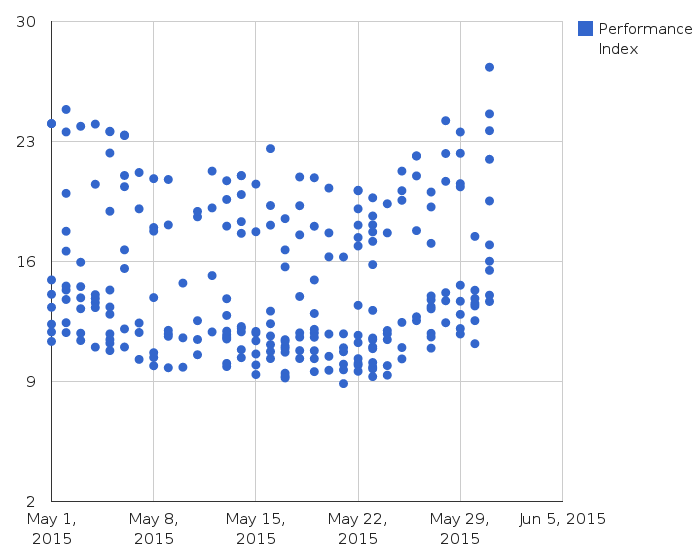
\includegraphics[scale=0.42]{media/performanceOverSellRange.png}
		\caption{Performance Index über Verkaufzeitraum}
		\end{figure}
		
		\begin{figure}[htp]
		\centering
		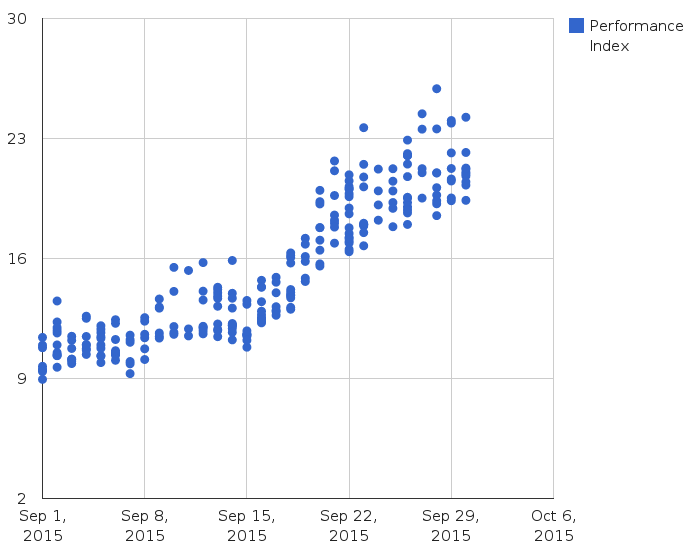
\includegraphics[scale=0.42]{media/performanceOverBuyRange.png}
		\caption{Performance Index über Verkaufzeitraum}
		\end{figure} 

	\printbibliography[heading=bibintoc,title={Quellenverzeichnis}]
	
    \chapter{Schlusserklärung}
        Ich erkläre, dass ich die Facharbeit ohne fremde Hilfe angefertigt und 
        nur die im Literaturverzeichnis angeführten Quellen und Hilfsmittel benutzt habe.
        
    

\end{document}
